\newpage
\begin{flushright}
    \section*{\Large{Ujian Tengah Semester}}
    \addcontentsline{toc}{section}{Ujian Tengah Semester (UTS)}
    \subsection*{Tahun 2020}
    \addcontentsline{toc}{subsection}{UTS - 2020}
\end{flushright}
\vspace{0.5cm}
\hrule height 2pt
\vspace{0.5cm}
\begin{center}
    \textbf{\large{MATERI}}
    \begin{enumerate}[leftmargin=*, label={\arabic*}.]
        \item Memahami konsep nilai mutlak
        \item Menyelesaikan pertidaksamaan yang melibatkan nilai mutlak.
        \item Mensketsa grafik fungsi.
        \item Fungsi komposisi dan menentukan domain dan rangenya.
        \item Mencari nilai limit kiri dan nilai limit kanan fungsi.
        \item Mencari nilai limit fungsi di tak hingga.
        \item Menentukan kekontinuan fungsi pada suatu titik.
        \item Menyelesaikan masalah turunan implisit.
        \item Menyelesaikan permasalahan maksimum dan minimum.
    \end{enumerate}
\end{center}
\vspace{0.2cm}
\hrule height 1pt
\vspace{0.5cm}
\begin{center}
    \textbf{\large{SOAL}}
\end{center}
\begin{enumerate}[leftmargin=*, label={\arabic*}.]
\item 
\begin{enumerate}[label={\alph*}.]
    \item Tentukanlah himpunan penyelesaian dari 
    $\ds \abs*{\frac{x}{x+2}} \geq x$.
    \item Jika terdapat persamaan yang menyatakan bahwa $|-a| = a$, 
    maka untuk nilai-nilai $a$ berapakah persamaan tersebut menjadi 
    benar atau salah?
\end{enumerate}
\item Diberikan fungsi 1 variabel bernilai real $f(x)$ dan $g(x)$ sebagai berikut:
\begin{center}
    $\ds f(x) = 
    \begin{cases}
        \abs{x+1}, &\text{jika $x < 1$}\\
        -x^{2}+4, &\text{jika $x \geq 1$}
    \end{cases}$ dan $\ds g(x) = \frac{1}{x}$
\end{center}
\begin{enumerate}[label={\alph*}.]
    \item Sketsalah grafik fungsi $f(x)$ dan $g(x)$ tanpa menggunakan bantuan
    \textit{software}.    
    \item Tentukanlah $(g \circ f)(x)$ sedemikian sehingga rumus fungsinya tidak 
    memuat nilai mutlak, kemudian tentukanlah domain dan range dari $(g \circ f)(x)$.
    \item Apakah 
    $\ds \floor*{(g \circ f)(0.5)} = \brk*{\frac{g \circ f}{g}}(0.5)$? 
    Jelaskanlah jawaban Anda!
\end{enumerate}
\item Diberikan fungsi $f\colon \mathbb{R} \to \mathbb{R}$ dengan $f(1)=f(-1)=1$ 
dan $\ds f(x) = \frac{x^{2}-x}{x^{2}-1}$ untuk $x$ lainnya.
\begin{enumerate}[label={\alph*}.]
    \item Hitunglah $\ds \lim_{x \to \infty} f(x)$ (jika ada)! 
    \item Hitunglah $\ds \lim_{x \to -\infty} f(x)$ (jika ada)! 
    \item Hitunglah $\ds \lim_{x \to 1} f(x)$ (jika ada)! 
    \item Hitunglah $\ds \lim_{x \to -1} f(x)$ (jika ada)!
    \item Apakah fungsi $f$ kontinu di titik $x=1$? Jelaskanlah! Jika $f$ tidak 
    kontinu di titik tersebut, apakah ketidakkontinuannya dapat diperbaiki? 
    Jelaskanlah! 
    \item Apakah fungsi $f$ kontinu di titik $x=-1$? Jelaskanlah! Jika $f$ tidak 
    kontinu di titik tersebut, apakah ketidakkontinuannya dapat diperbaiki? 
    Jelaskanlah! 
\end{enumerate}
\item 
\begin{enumerate}[label={\alph*}.]
    \item Tentukanlah persamaan garis singgung yang menyinggung kurva \\
    $xy^{2}+y(x^{2}+1)^{2} = y^{2}+x$ di titik $(0,1)$.
    \item Tentukanlah turunan kedua dari fungsi implisit di soal sebelumnya 
    pada titik $(0,1)$.
\end{enumerate}
\item Tentukanlah panjang dan lebar suatu persegi panjang yang bisa dimasukkan 
kedalam elips dengan persamaan $\ds \frac{x^{2}}{a}+\frac{y^{2}}{b}=1$ 
sedemikian sehingga luas persegi panjang tersebut maksimum.
\end{enumerate}
\vspace{0.2cm}
\hrule height 1pt
\vspace{0.5cm}
\begin{center}
    \textbf{\large{PEMBAHASAN}}
\end{center}
\begin{enumerate}[leftmargin=*, label={\arabic*}.]
\item
\begin{enumerate}[label={\alph*}.]
    \item Akan dicari himpunan penyelesaian dari 
    $\ds \abs*{\frac{x}{x+2}} \geq x$.\\
    Hanya ada 3 aturan dasar yang diperlukan untuk menyelesaikan pertidaksamaan.
    \begin{enumerate}[label={\arabic*})]
        \item Jumlahkan kedua ruas dengan bilangan yang sama.
        \item Kalikan kedua ruas dengan bilangan positif yang sama.
        \item Kalikan kedua ruas dengan bilangan negatif yang sama dan 
        mengubah arah pertidaksamaannya.
    \end{enumerate}
    Pada soal ini ruas kiri melibatkan nilai mutlak. Untuk menyelesaikannya 
    pertidaksamaan perlu diubah kebentuk yang tidak melibatkan nilai mutlak. 
    Cara yang selalu bisa digunakan adalah dengan membagi kasus pada nilai $x$.
        
    Perhatikan bahwa sesuai definisi nilai mutlak
    \[
    \abs*{\frac{x}{x+2}} = 
    \begin{cases}
        \frac{x}{x+2}, &\text{jika $\frac{x}{x+2} \geq 0$ atau $x < -2 \cup x \geq 0$ $^{*1}$}\\
        -\frac{x}{x+2}, &\text{jika $\frac{x}{x+2} < 0$ atau $-2 < x < 0$ $^{*2}$}
    \end{cases}
    \]
    (*1) $\frac{x}{x+2} \geq 0$ dapat disederhanakan dengan menyelesaikan 
    pertidaksamaannya. \\Titik stasioner pertidaksamaan ini adalah $x= 0$ dan $x=-2$.
    \begin{center}
    \begin{tikzpicture}
        \draw[stealth-stealth] (-5,0) node[below]{$-\infty$}--(5,0) node[below]{$\infty$};
        \draw (-5,1) --(-2,1);
        \draw (2,1) --(5,1);
        \draw (-2,1)--(-2,-.1) node[below=0.2em]{$-2$};
        \draw (2,1)--(2,-.1) node[below=0.2em]{$0$};
                
        \node at (3.5,.5) {$+$};
        \node at (-4,.5) {$+$};
        \node at (0,.5) {$-$};
        \node [draw, shape = circle, fill = black, minimum size = 0.1cm, inner sep=0pt] at (2,0){};
        \node [draw, shape = circle, fill = white, minimum size = 0.1cm, inner sep=0pt] at (-2,0){};
    \end{tikzpicture}
    \end{center}
    Sehingga
    \[
        \frac{x}{x+2} \geq 0 \iff x < -2 \cup x \geq 0
    \]
    (*2) $\frac{x}{x+2} < 0$ dengan gambaran garis bilangan yang sama seperti sebelumnya
    \[
        \frac{x}{x+2} < 0 \iff -2 < x < 0
    \]
    Sehingga pertidaksamaan ini diselesaikan dengan membagi menjadi 2 kasus seperti 
yang terlihat pada garis bilangan di bawah ini.

\vspace{0.2cm}
\begin{tikzpicture}
\draw[stealth-stealth] (-6,0) node[below]{$-\infty$}--(5,0) node[below]{$\infty$};
\draw (-2,.1)--(-2,-.1) node[below=0.2em]{$-2$};
\draw (1,.1)--(1,-.1) node[below=0.2em]{$0$};
\node at (-7,.7) {$\ds \abs*{\frac{x}{x+2}}=$};

\node at (-4,.7) {$\ds \frac{x}{x+2}$};
\node at (-.5,.7) {$\ds -\frac{x}{x+2}$};
\node at (3,.7) {$\ds \frac{x}{x+2}$};
\end{tikzpicture}

\textbf{Kasus 1: $x < -2 \cup x \geq 0$}\\
Maka
\begin{align*}
    \abs*{\frac{x}{x+2}} \geq x
    \iff &\frac{x}{x+2} \geq x
    &\text{definisi nilai mutlak} \\
    \iff &\frac{x}{x+2} -x \geq 0
    &\text{kedua ruas jumlahkan $-x$}\\
    \iff &\frac{-x^{2}-x}{x+2} \geq 0
    &\text{penyederhanaan}\\
    \iff &\frac{x^{2}+x}{x+2} \leq 0
    &\text{kedua ruas kalikan $-1$}\\
    \iff &\frac{x(x+1)}{x+2} \leq 0
    &\text{faktorisasi}\\
\end{align*}
Titik stasioner pertidaksamaan ini adalah $x=-2$, $x=-1$, dan $x=0$.
\begin{center}
    \begin{tikzpicture}
        \draw[stealth-stealth] (-5,0) node[below]{$-\infty$}--(5,0) node[below]{$\infty$};
        \draw (-5,1) --(-2,1);
        \draw (0,1) --(2,1);
        \draw (-2,1)--(-2,-.1) node[below=0.2em]{$-2$};
        \draw (0,1)--(0,-.1) node[below=0.2em]{$-1$};
        \draw (2,1)--(2,-.1) node[below=0.2em]{$0$};
                
        \node at (3.5,.5) {$+$};
        \node at (-4,.5) {$-$};
        \node at (1,.5) {$-$};
        \node at (-1,.5) {$+$};
        \node [draw, shape = circle, fill = black, minimum size = 0.1cm, inner sep=0pt] at (2,0){};
        \node [draw, shape = circle, fill = black, minimum size = 0.1cm, inner sep=0pt] at (0,0){};
        \node [draw, shape = circle, fill = white, minimum size = 0.1cm, inner sep=0pt] at (-2,0){};
    \end{tikzpicture}
\end{center}
Sehingga nilai $x$ yang memenuhi pertidaksamaan adalah $x < -2 \cup -1 \leq x \leq 0$. Ambil 
irisannya dengan syarat pada kasus ini maka himpunan penyelesaian pada kasus ini adalah 
\\$\set{x < -2 \, \cup \, x = 0}$. 

\textbf{Kasus 2: $-2 < x < 0$}\\
Maka
\begin{align*}
    \abs*{\frac{x}{x+2}} \geq x
    \iff &-\frac{x}{x+2} \geq x
    &\text{definisi nilai mutlak} \\
    \iff &-\frac{x}{x+2} -x \geq 0
    &\text{kedua ruas jumlahkan $-x$}\\
    \iff &\frac{-x^{2}-3x}{x+2} \geq 0
    &\text{penyederhanaan}\\
    \iff &\frac{x^{2}+3x}{x+2} \leq 0
    &\text{kedua ruas kalikan $-1$}\\
    \iff &\frac{x(x+3)}{x+2} \leq 0
    &\text{faktorisasi}\\
\end{align*}
Titik stasioner pertidaksamaan ini adalah $x=-3$, $x=-2$, dan $x=0$.
\begin{center}
    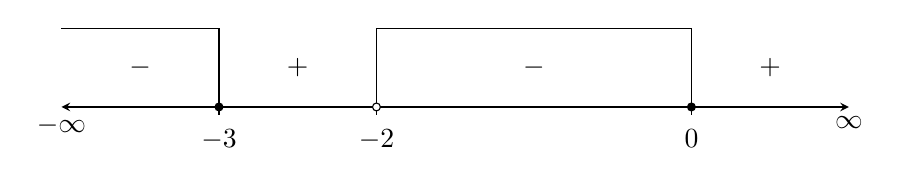
\begin{tikzpicture}
        \draw[stealth-stealth] (-5,0) node[below]{$-\infty$}--(5,0) node[below]{$\infty$};
        \draw (-5,1) --(-3,1);
        \draw (-1,1) --(3,1);
        \draw (-1,1)--(-1,-.1) node[below=0.2em]{$-2$};
        \draw (-3,1)--(-3,-.1) node[below=0.2em]{$-3$};
        \draw (3,1)--(3,-.1) node[below=0.2em]{$0$};
                
        \node at (4,.5) {$+$};
        \node at (-4,.5) {$-$};
        \node at (1,.5) {$-$};
        \node at (-2,.5) {$+$};
        \node [draw, shape = circle, fill = black, minimum size = 0.1cm, inner sep=0pt] at (3,0){};
        \node [draw, shape = circle, fill = black, minimum size = 0.1cm, inner sep=0pt] at (-3,0){};
        \node [draw, shape = circle, fill = white, minimum size = 0.1cm, inner sep=0pt] at (-1,0){};
    \end{tikzpicture}
\end{center}
Sehingga nilai $x$ yang memenuhi pertidaksamaan adalah $x \leq -3 \cup -2 < x \leq 0$. Ambil 
irisannya dengan syarat pada kasus ini maka himpunan penyelesaian pada kasus ini adalah 
\\$\set{-2 < x < 0}$. 

Himpunan penyelesaiannya adalah gabungan semua nilai $x$ yang memenuhi pertidaksamaan. 
Sehingga himpunan tersebut adalah 
$\set*{x < -2 \cup x = 0 \cup -2 < x < 0}$ 
atau \\
$\set*{x \in \mathbb{R} \mid x < -2 \cup -2 < x \leq 0}$
atau
$\oic*{-\infty,0} \cap \set{x \in \mathbb{R} \mid x \neq 2}$

$\therefore$ Himpunan penyelesaian dari 
$\ds \abs*{\frac{x}{x+2}} \geq x$ adalah 
$\set*{x \in \mathbb{R} \mid x < -2 \cup -2 < x \leq 0}$
atau \\
$\oic*{-\infty,0} \cap \set{x \in \mathbb{R} \mid x \neq 2}$

\vspace{0.1cm}
\textbf{Catatan:}\\
Salah satu cara untuk mengubah pertidaksamaan yang melibatkan nilai mutlak ke 
pertidaksamaan yang tidak adalah dengan menguadratkan kedua ruas. Soal ini \textbf{TIDAK} 
dapat diselesaikan dengan cara tersebut. Hal ini dikarenakan cara tersebut memiliki syarat 
yaitu kedua ruasnya harus bernilai positif.
\begin{center}
    \line(1,0){150}
\end{center}
\item Diberikan persamaan $\abs{-a} = a$, akan dicari interval dimana nilai $a$ menghasilkan
persamaan yang benar dan persamaan yang salah.\\
Menggunakan definisi nilai mutlak maka
\[
    \abs{-a} = 
    \begin{cases}
        -a, &-a \geq 0 \iff a \leq 0\\
        -(-a), &-a < 0 \iff a > 0
    \end{cases}
\]
\textbf{Kasus 1: $a \leq 0$}\\
Maka $\abs{-a} = a \iff -a = a$. Persamaan ini benar hanya saat $a = 0$.\\
Sehingga untuk $a < 0$ persamaan ini menjadi salah sedangkan $a = 0$ menjadi benar.\\
\textbf{Kasus 2: $a > 0$}\\
Maka $\abs{-a} = a \iff -(-a) = a \iff a = a$. Persamaan ini 
selalu benar. Sehingga untuk $a > 0$, persamaan ini menjadi benar.

$\therefore$ Persamaan ini bernilai benar untuk $a \geq 0$ dan bernilai salah untuk $a < 0$.
\end{enumerate}
\begin{center}
    \line(1,0){300}
\end{center}
\item Diberikan
\begin{center}
    $\ds f(x) = 
    \begin{cases}
        \abs{x+1}, &\text{jika $x < 1$}\\
        -x^{2}+4, &\text{jika $x \geq 1$}
    \end{cases}$ dan $\ds g(x) = \frac{1}{x}$
\end{center}
\begin{enumerate}[label={\alph*}.]
    \item Akan disketsa grafik fungsi $f$ dan $g$\\
    3 tahap sketsa grafik adalah:
    \begin{enumerate}[label={\arabic*})]
        \item Cari beberapa titik koordinat $(x,f(x))$.
        \item Plot titik pada bidang
        \item Hubungkan titik-titik menjadi sebuah kurva
    \end{enumerate}
    Karena $f$ adalah fungsi \textit{pointwise} maka dibagi menjadi 2 bagian, saat
    $x < 1$ dan $x \geq 1$.\\
    Untuk $x < 1$, $f(x) = |x+1|$ cari titik dimana $|x+1|=0$ dan dua titik di kiri 
    dan kanannya. Berikut hasilnya dalam tabel.
    \begin{center}
    \begin{tabular}{|c|c|c|c|}\hline
        $x$ & $-2$ & $-1$ & $0$ \\ \hline
        $f(x)$ & $1$ & $0$ & $1$ \\ \hline
    \end{tabular}
    \end{center}
    Untuk $x \geq 1$, karena fungsinya kuadratik, cari tiga titik berbeda (sifat interpolasi).
    Berikut hasilnya dalam tabel.
    \begin{center}
    \begin{tabular}{|c|c|c|c|}\hline
        $x$ & $1$ & $2$ & $3$ \\ \hline
        $f(x)$ & $3$ & $0$ & $-5$ \\ \hline
    \end{tabular}
    \end{center}

Plot keenam titik tersebut dalam bidang kartesian dan hubungkan sehingga diperolah grafik 
seperti berikut.
\begin{center}
\begin{tikzpicture}[>=stealth]
\begin{axis}[
    xmin=-4,xmax=4,
    ymin=-6,ymax=4,
    axis x line=middle,
    axis y line=middle,
    axis line style=<->,
    xlabel={$x$},
    ylabel={$f(x)$},
    ]
    \addplot[no marks,blue, <-] expression[domain=-3:1,samples=100]{abs(x+1)} 
        node[pos=0,anchor=south west]{$\abs{x+1}$};
    \addplot[no marks,blue, ->] expression[domain=1:3.1,samples=100]{-x^2+4} 
        node[pos=0.25,anchor=south west]{$-x^{2}+4$}; 
    \node [draw, shape = circle, fill = white, minimum size = 0.1cm, inner sep=0pt] at (1,2){};
    \node [draw, shape = circle, fill = black, minimum size = 0.1cm, inner sep=0pt] at (1,3){};
    \node [draw, shape = circle, fill = black, minimum size = 0.1cm, inner sep=0pt] at (2,0){};
    \node [draw, shape = circle, fill = black, minimum size = 0.1cm, inner sep=0pt] at (3,-5){};
    \node [draw, shape = circle, fill = black, minimum size = 0.1cm, inner sep=0pt] at (-2,1){};
    \node [draw, shape = circle, fill = black, minimum size = 0.1cm, inner sep=0pt] at (-1,0){};
    \node [draw, shape = circle, fill = black, minimum size = 0.1cm, inner sep=0pt] at (0,1){};
\end{axis}
\end{tikzpicture}
\end{center}
Untuk $g(x) = \frac{1}{x}$ adalah fungsi spesial yang sangat disarankan untuk diingat bentuk grafiknya. 
Cara yang sama dapat dilakukan (Uji tiga titik saat $x < 0$ dan tiga titik saat $x > 0$)
\begin{center}
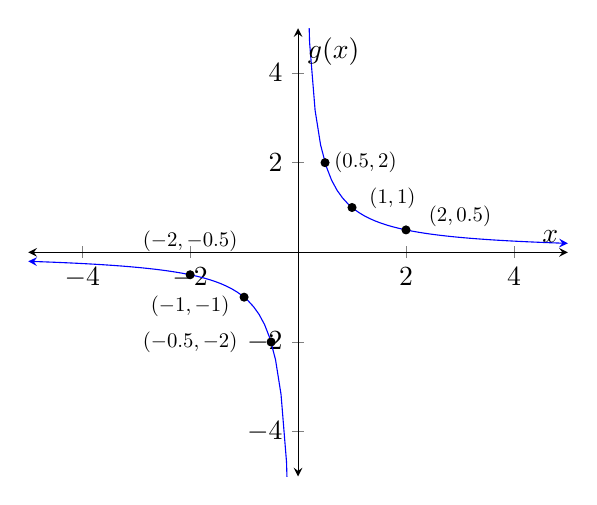
\begin{tikzpicture}[>=stealth]
\begin{axis}[
    xmin=-5,xmax=5,
    ymin=-5,ymax=5,
    axis x line=middle,
    axis y line=middle,
    axis line style=<->,
    xlabel={$x$},
    ylabel={$g(x)$},
    ]
    \addplot[no marks,blue, <-] expression[domain=-5:-0.01,samples=50]{1/x} 
        node[pos=0,anchor=south west]{};
    \addplot[no marks,blue, ->] expression[domain=0.01:5,samples=50]{1/x} 
        node[pos=0,anchor=south west]{};
    \node [draw, shape = circle, fill = black, minimum size = 0.1cm, inner sep=0pt] at (0.5,2){};
    \node [draw, shape = circle, fill = black, minimum size = 0.1cm, inner sep=0pt] at (1,1){};
    \node [draw, shape = circle, fill = black, minimum size = 0.1cm, inner sep=0pt] at (2,0.5){};
    \node at (1.25,2) {\scalebox{0.75}{$(0.5,2)$}};
    \node at (1.75,1.2) {\scalebox{0.75}{$(1,1)$}};
    \node at (3,0.8) {\scalebox{0.75}{$(2,0.5)$}};
    \node [draw, shape = circle, fill = black, minimum size = 0.1cm, inner sep=0pt] at (-0.5,-2){};
    \node [draw, shape = circle, fill = black, minimum size = 0.1cm, inner sep=0pt] at (-1,-1){};
    \node [draw, shape = circle, fill = black, minimum size = 0.1cm, inner sep=0pt] at (-2,-0.5){};
    \node at (-2,-2) {\scalebox{0.75}{$(-0.5,-2)$}};
    \node at (-2,-1.2) {\scalebox{0.75}{$(-1,-1)$}};
    \node at (-2,0.25) {\scalebox{0.75}{$(-2,-0.5)$}};
\end{axis}
\end{tikzpicture}
\end{center}
$\therefore$ Telah disketsa grafik $f$ dan $g$ seperti gambar diatas.
\begin{center}
    \line(1,0){150}
\end{center}
\item Akan dicari $(g \circ f)(x)$ sehingga fungsinya tidak memuat nilai mutlak.\\
Nilai mutlak berasal dari fungsi $f$ ketika $x < 1$, nilai mutlak ini dapat dihilangkan 
dengan menjabarkan kasus dari nilai mutlak. Sesuai definisi nilai mutlak:
\[
    \abs{x+1} =
    \begin{cases}
    x+1, &x+1 \geq 0 \iff x \geq -1,\\
    -(x+1), &x+1 < 0 \iff x < -1
    \end{cases}
\]
dengan demikian fungsi $f$ dapat diubah menjadi
\[
    f(x) = 
    \begin{cases}
        -(x+1), & x < -1,\\
        x+1, &-1 \leq x < 1,\\
        -x^{2}+4, &x \geq 1.
    \end{cases}
\]
sehingga fungsi komposisi $(g \circ f)(x)$ adalah
\[
    (g\circ f)(x) = g(f(x)) = 
    \begin{cases}
        \frac{1}{-(x+1)}, & x < -1,\\
        \frac{1}{x+1}, &-1 \leq x < 1 \quad ^*(x \neq -1),\\
        \frac{1}{-x^{2}+4}, &x \geq 1 \quad ^*(x \neq 2).
    \end{cases}
\]
Selanjutnya akan dicari domain dari $(g \circ f)(x)$. \\
Domain dari $(g \circ f)(x)$ adalah irisan dari domain $f$ dengan domain dari setiap kasus 
pada fungsi \textit{pointwise} $(g \circ f)(x)$. Fungsi $f$ hanya 
melibatkan bentuk linear dan kuadratik, sehingga domainnya adalah $\mathbb{R}$.\\

Domain dari $\ds \frac{1}{-(x+1)}$.

Karena melibatkan bentuk rasional maka $-(x+1) \neq 0 \iff x \neq -1$. Karena 
syarat kasus ini $x < -1$ maka domainnya adalah $x < -1$.

Domain dari $\ds \frac{1}{x+1}$.

Karena melibatkan bentuk rasional maka $x+1 \neq 0 \iff x \neq -1$. Karena 
syarat kasus ini $-1 \leq x < 1$, maka domainnya adalah $-1 < x < 1$.

Domain dari $\ds \frac{1}{-x^{2}+4}$.

Karena melibatkan bentuk rasional maka $-x^{2}+4 \neq 0 \iff x \neq -2,2$.\\
Karena syarat kasus ini $x \geq 1$, maka domainnya adalah $x \geq 1 \cap x \neq 2$.\\
Bila digabung maka domain dari $(g \circ f)(x)$ adalah 
$\set*{x \in \mathbb{R} \mid x \neq -1, x\neq 2}$ \\

Terakhir akan dicari range dari $(g \circ f)(x)$.

Dari kasus $\ds \frac{1}{-x^{2}+4}$ 
karena $\ds \lim_{x\to 2^{+}} (g \circ f)(x) = -\infty$ dan 
$\ds \lim_{x\to \infty} (g \circ f)(x) = 0$ maka 
$\oio{-\infty,0}$ adalah bagian dari range $g \circ f$.\\
Dari kasus $\ds \frac{1}{-(x+1)}$ 
karena $\ds \lim_{x\to -1^{-}} (g \circ f)(x) = \infty$ dan 
$\ds \lim_{x\to -\infty} (g \circ f)(x) = 0$ maka 
$\oio{0,\infty}$ adalah bagian dari range $g \circ f$.

Sehingga range dari $g \circ f$ sudah mencakup semua bilangan real kecuali $0$.
Dan karena $g \circ f$ berbentuk rasional dengan penyebut bernilai satu maka $0$ 
tidak bisa menjadi hasil dari $g \circ f$.

Dengan demikian range dari $(g \circ f)(x)$ adalah $\oio{-\infty,\infty} \cap x \neq 0$ 
atau $\set{y \in \mathbb{R} \mid y \neq 0}$.

Berikut grafik pendukung.

\begin{center}
\begin{tikzpicture}[>=stealth]
\begin{axis}[
    xmin=-5,xmax=5,
    ymin=-5,ymax=5,
    axis x line=middle,
    axis y line=middle,
    axis line style=<->,
    xlabel={$x$},
    ylabel={$(g \circ f)(x)$},
    ]
    \addplot[no marks,blue, <-] expression[domain=-5:1,samples=99]{1/abs(x+1)} 
        node[pos=0,anchor=south west]{};
    \addplot[no marks,blue, -] expression[domain=1:1.99,samples=20]{1/(-x^2+4)} 
        node[pos=0,anchor=south west]{};
    \addplot[no marks,blue, ->] expression[domain=2.01:5,samples=80]{1/(-x^2+4)} 
        node[pos=0,anchor=south west]{};
    \node [draw, shape = circle, fill =  white, minimum size = 0.08cm, inner sep=0pt] at (1,0.5){};
    \node [draw, shape = circle, fill = blue, minimum size = 0.08cm, inner sep=0pt] at (1,1/3){};  
\end{axis}
\end{tikzpicture}
\end{center}

$\therefore$ 
\[
    (g\circ f)(x) = g(f(x)) = 
    \begin{cases}
        \frac{1}{-(x+1)}, & x < -1,\\
        \frac{1}{x+1}, &-1 < x < 1 \\
        \frac{1}{-x^{2}+4}, &x > 1,\,x \neq 2.
    \end{cases}
\]
dengan domain $\set*{x \in \mathbb{R} \mid x \neq -1, x\neq 2}$ dan range
$\set{y \in \mathbb{R} \mid y \neq 0}$.
\begin{center}
    \line(1,0){150}
\end{center}
\item Akan diuji kebenaran dari 
$\ds \floor*{(g \circ f)(0.5)} = \brk*{\frac{g \circ f}{g}}(0.5)$.

Evaluasi nilai $\floor*{(g \circ f)(0.5)}$.
\begin{align*}
    \floor*{(g \circ f)(0.5)}
    &= \floor*{g(f(0.5))}
    &\text{definisi komposisi} \\
    &= \floor*{g(abs{0.5+1})} 
    &\text{evaluasi fungsi $f$} \\
    &= \floor*{g(1.5)}
    &\text{penyederhanaan}\\
    &=\floor*{\frac{1}{1.5}}
    &\text{evaluasi fungsi $g$}\\
    &=0 
    &\text{evaluasi $floor$}
\end{align*}

Evaluasi nilai $\ds \brk*{\frac{g \circ f}{g}}(0.5)$
\begin{align*}
    \brk*{\frac{g \circ f}{g}}(0.5) &= \frac{(g\circ f)(0.5)}{g(0.5)}\\
    &= \frac{g(f(0.5))}{g(0.5)} 
    &\text{definisi komposisi}\\
    &= \frac{g(\abs{0.5+1})}{g(0.5)}
    &\text{evaluasi fungsi $f$} \\
    &= \frac{g(1.5)}{g(0.5)} 
    &\text{penyederhanaan}\\
    &= \frac{1/1.5}{1/0.5}
    &\text{evaluasi fungsi $g$}\\
    &=\frac{0.5}{1.5} = \frac{1}{3}
    &\text{penyederhanaan}
\end{align*}
Diperoleh 
\[
    \floor*{(g \circ f)(0.5)} = 0 \neq \frac{1}{3} = \brk*{\frac{g \circ f}{g}}(0.5)
\]

$\therefore$ 
$\ds \floor*{(g \circ f)(0.5)} \neq \brk*{\frac{g \circ f}{g}}(0.5)$
\end{enumerate}
\begin{center}
    \line(1,0){300}
\end{center}
\item Diberikan fungsi $f\colon \mathbb{R} \to \mathbb{R}$ dengan $f(1)=f(-1)=1$ 
dan $\ds f(x) = \frac{x^{2}-x}{x^{2}-1}$ untuk $x$ lainnya.
\begin{enumerate}[label={\alph*}.]
    \item Akan dicari $\ds \lim_{x \to \infty} f(x)$ (jika ada).
    \begin{align*}
        \lim_{x \to \infty} f(x) 
        &= \lim_{x \to \infty} \frac{x^{2}-x}{x^{2}-1}
        &\text{karena fungsi mendekati $\infty$}\\
        &= \lim_{x \to \infty} \frac{1-\frac{1}{x}}{1-\frac{1}{x^{2}}}
        &\text{kalikan $\frac{1/x^{2}}{1/x^{2}}$ (karena $x \neq 0$)}\\
        &=\frac{\lim_{x \to \infty} 1 - \lim_{x \to \infty} \frac{1}{x}}
        {\lim_{x \to \infty} 1 - \lim_{x \to \infty}\frac{1}{x^{2}}}
        &\text{teorema utama limit}\\
        &= \frac{\lim_{x \to \infty} 1 - 0}{\lim_{x \to \infty} 1 - 0}
        &\text{karena $\lim_{x\to\infty}\frac{1}{x} = \lim_{x\to\infty}\frac{1}{x^{2}} = 0$}\\
        &= \frac{1}{1} = 1
        &\text{teorema utama limit}
    \end{align*} 
    $\therefore$ $\ds \lim_{x \to \infty} f(x)$ ada dan 
    $\ds \lim_{x \to \infty} f(x) = 1$
\begin{center}
    \line(1,0){150}
\end{center}
    \item Akan dicari $\ds \lim_{x \to -\infty} f(x)$ (jika ada).
    \begin{align*}
        \lim_{x \to -\infty} f(x) 
        &= \lim_{x \to -\infty} \frac{x^{2}-x}{x^{2}-1}
        &\text{karena fungsi mendekati $-\infty$}\\
        &= \lim_{x \to -\infty} \frac{1-\frac{1}{x}}{1-\frac{1}{x^{2}}}
        &\text{kalikan $\frac{1/x^{2}}{1/x^{2}}$ (karena $x \neq 0$)}\\
        &=\frac{\lim_{x \to -\infty} 1 - \lim_{x \to -\infty} \frac{1}{x}}
        {\lim_{x \to- \infty} 1 - \lim_{x \to -\infty}\frac{1}{x^{2}}}
        &\text{teorema utama limit}\\
        &= \frac{\lim_{x \to -\infty} 1 - 0}{\lim_{x \to -\infty} 1 - 0}
        &\text{karena $\lim_{x\to -\infty}\frac{1}{x} = \lim_{x\to -\infty}\frac{1}{x^{2}} = 0$}\\
        &= \frac{1}{1} = 1
        &\text{teorema utama limit}
    \end{align*} 
    $\therefore$ $\ds \lim_{x \to -\infty} f(x)$ ada dan 
    $\ds \lim_{x \to -\infty} f(x) = 1$
\begin{center}
\line(1,0){150}
\end{center}
    \item Akan dicari $\ds \lim_{x \to 1} f(x)$ (jika ada).
    \begin{align*}
        \lim_{x \to 1} f(x) 
        &= \lim_{x \to 1} \frac{x^{2}-x}{x^{2}-1}
        &\text{karena fungsi mendekati $1$}\\
        &= \lim_{x \to 1} \frac{x(x-1)}{(x+1)(x-1)}
        &\text{faktorisasi}\\
        &=\lim_{x \to 1} \frac{x}{x+1}
        &\text{kalikan $\frac{1/(x-1)}{1/(x-1)}$ (karena $x \neq 1$)}\\
        &= \frac{1}{1+1} = \frac{1}{2} 
        &\text{teorema subtitusi}
    \end{align*} 
    $\therefore$ $\ds \lim_{x \to 1} f(x)$ ada dan 
    $\ds \lim_{x \to 1} f(x) = \frac{1}{2}$
\begin{center}
\line(1,0){150}
\end{center}    
    \item Akan dibuktikan $\ds \lim_{x \to -1} f(x)$ tidak ada.\\
    Gunakan limit kiri atau limit kanannya.
    \begin{align*}
        \lim_{x \to -1^{-}} f(x) 
        &= \lim_{x \to -1^{-}} \frac{x^{2}-x}{x^{2}-1}
        &\text{karena fungsi mendekati $1$}\\
        &= \lim_{x \to -1^{-}} \frac{x(x-1)}{(x+1)(x-1)}
        &\text{faktorisasi}\\
        &= \lim_{x \to -1^{-}} \frac{x}{x+1}
        &\text{kalikan $\frac{1/(x-1)}{1/(x-1)}$ (karena $x \neq 1$)}\\
        &= -\infty
    \end{align*} 
    Karena limit kirinya tidak ada, maka limitnya juga tidak ada.

    $\therefore$ $\ds \lim_{x \to -1} f(x)$ tidak ada. 
\begin{center}
\line(1,0){150}
\end{center}    
    Untuk soal e dan f, $f$ kontinu di $c$ jika
    \begin{enumerate}[label={\arabic*}.]
        \item $\lim_{x\to c} f(x)$ ada.
        \item $f(c)$ ada.
        \item $\lim_{x\to c} f(x) = f(c)$
    \end{enumerate}
    \item Akan dibuktikan $f$ tidak kontinu di $x = 1$.\\
    Hal ini karena dari informasi soal, dan hasil poin c sebelumnya,
    \[
        \lim_{x\to 1} f(x) = \frac{1}{2} \neq 1 = f(1)
    \]
    Kekontinuannya dapat diperbaiki dengan mendefinisikan ulang nilai $f(1)$ 
    menjadi nilai limitnya.

    $\therefore$ $f$ tidak kontinu di $x=1$ dan dapat diperbaiki.
\begin{center}
\line(1,0){150}
\end{center} 
    \item Akan dibuktikan $f$ tidak kontinu di $x = -1$.\\
    Hal ini karena dari hasil poin d sebelumnya, $\lim_{x\to -1} f(x)$ 
    tidak ada.
    Kekontinuannya tidak dapat diperbaiki karena limitnya tidak ada di $x=-1$.

    $\therefore$ $f$ tidak kontinu di $x=-1$ dan tidak dapat diperbaiki.
\end{enumerate}
\begin{center}
    \line(1,0){300}
\end{center}
\item 
\begin{enumerate}[label={\alph*}.]
    \item Akan dicari persamaan garis singgung yang menyinggung kurva \\
    $xy^{2}+y(x^{2}+1)^{2} = y^{2}+x$ di titik $(0,1)$.\\
    Untuk memperoleh persamaan garis diperlukan kemiringan garis dan satu titik
    di dalam garis. Titik $(0,1)$ ada pada garis singgung sehingga tinggal mencari 
    kemiringannya. Kemiringannya akan sama dengan turunan pertama $(y')$ kurva di titik 
    $(0,1)$. Akan dicari turunan pertama kurva.

    Gunakan turunan implisit
    \begin{align*}
        \drv{x}{xy^{2}+y(x^{2}+1)^{2}} = \drv{x}{y^{2}+x} \iff 
        \drv{x}{xy^{2}} + \drv{x}{y(x^{2}+1)^{2}} = \drv{x}{y^{2}} + \drv{x}{x}
    \end{align*}
    Karena persamaan akan panjang dan memakan tempat, selesaikan masing-masing nilai 
    turunan.
    \begin{enumerate}[label={\arabic*})]
        \item 
        \begin{align*}
            \drv{x}{xy^{2}} 
            &= \drv{x}{x}y^{2}+x\drv{x}{y^{2}}
            &\text{aturan perkalian}\\
            &= (1)y^{2} + x(2yy') = y^{2} + 2xyy'
        \end{align*}
        \item 
        \begin{align*}
            \drv{x}{y(x^{2}+1)^{2}} 
            &= \drv{x}{y}(x^{2}+1)^{2}+y\drv{x}{(x^{2}+1)^{2}}
            &\text{aturan perkalian}\\
            &= y'(x^{2}+1)^{2} + y\drv{x}{(x^{2}+1)^{2}}\\
            &=y'(x^{2}+1)^{2} + y\brk*{2(x^{2}+1)\drv{x}{x^{2}+1}}
            &\text{aturan pangkat dan rantai}\\
            &=y'(x^{2}+1)^{2} + y\brk*{2(x^{2}+1)(2x)}\\
            &=y'(x^{2}+1)^{2} + 4xy(x^{2}+1)
        \end{align*}
        \item 
        \[
            \drv{x}{y^{2}} = 2y\drv{x}{y} = 2yy' \quad \text{aturan rantai}
        \]
    \end{enumerate}
    Sehingga 
    \begin{align*}
        &\drv{x}{xy^{2}} + \drv{x}{y(x^{2}+1)^{2}} = \drv{x}{y^{2}} + \drv{x}{x} \\
        \iff &\brk*{y^{2} + 2xyy'} + \brk*{y'(x^{2}+1)^{2} 
        + 4xy(x^{2}+1)}= 2yy' + 1\\
    \end{align*}
    Subtitusi $x = 0$ dan $y=1$ untuk memperoleh turunan pertama kurva di $(0,1)$.
    \begin{align*}
        &\brk*{y^{2} + 2xyy'} + \brk*{y'(x^{2}+1)^{2} 
        + 4xy(x^{2}+1)}= 2yy' + 1\\
        \iff &\brk*{1^{2} + 2(0)(1)y'} + \brk*{y'(0^{2}+1)^{2} 
        + 4(0)(1)(x^{2}+1)}= 2(1)
        y' + 1\\
        \iff &1+0+y'+0 = 2y'+1\\
        \iff &-y' = 0 \iff y' = 0
    \end{align*}
    Maka kemiringan garis singgung adalah $m = y' = 0$ dan diperoleh garis singgung
    \begin{align*}
        y-y_1 &= m(x-x_1)\\
        y-1 &= 0(x-0)\\
        y &= 1
    \end{align*}

    $\therefore$ Persamaan garis singgung yang menyinggung kurva \\
    $xy^{2}+y(x^{2}+1)^{2} = y^{2}+x$ di titik $(0,1)$ adalah $y=1$
    \item Akan dicari turunan kedua dari fungsi implisit di soal sebelumnya 
    pada titik $(0,1)$. Dari soal sebelumnya, setelah 1 kali penurunan secara 
    implisit diperoleh
    \[
        \brk*{y^{2} + 2xyy'} + \brk*{y'(x^{2}+1)^{2} 
        + 4xy(x^{2}+1)}= 2yy' + 1
    \]
    Turunkan lagi secara implisit persamaan ini, yaitu
    \[
        \drv{x}{y^{2}}+\drv{x}{2xyy'}+\drv{x}{y'(x^{2}+1)^{2}}+\drv{x}{4xy(x^{2}+1)}
        =\drv{x}{2yy'}+\drv{x}{1}
    \]
    Karena persamaan akan panjang dan memakan tempat, selesaikan masing-masing nilai 
    turunan.
    \begin{enumerate}[label={\arabic*})]
        \item 
        \[
            \drv{x}{y^{2}} = 2y\drv{x}{y} = 2yy' \quad \text{aturan rantai}
        \]
        \item 
        \begin{align*}
            \drv{x}{(2xy)y'} 
            &= \drv{x}{2xy}y' + 2xy\drv{x}{y'}
            &\text{aturan perkalian}\\
            &= \drv{x}{2xy}y' + 2xyy''\\
            &= \brk*{\drv{x}{2x}y + 2x\drv{x}{y}}y' + 2xyy''
            &\text{aturan perkalian}\\
            &=(2y+2xy')y'+2xyy''
        \end{align*}
        \item 
        \begin{align*}
            \drv{x}{y'(x^{2}+1)^{2}} 
            &= \drv{x}{y'}(x^{2}+1)^{2}+y'\drv{x}{(x^{2}+1)^{2}}
            &\text{aturan perkalian}\\
            &= y''(x^{2}+1)^{2} + y'\drv{x}{(x^{2}+1)^{2}}\\
            &=y''(x^{2}+1)^{2} + y'\brk*{2(x^{2}+1)\drv{x}{x^{2}+1}}
            &\text{aturan pangkat dan rantai}\\
            &=y''(x^{2}+1)^{2} + y'\brk*{2(x^{2}+1)(2x)}\\
            &=y''(x^{2}+1)^{2} + 4xy'(x^{2}+1)
        \end{align*}
        \item 
        \begin{align*}
            \drv{x}{(4xy)(x^{2}+1)}
            &=\drv{x}{4xy}(x^{2}+1) + (4xy)\drv{x}{x^{2}+1}
            &\text{aturan perkalian}\\
            &=\drv{x}{4xy}(x^{2}+1) + (4xy)(2x)\\
            &=\drv{x}{4xy}(x^{2}+1) + 8x^{2}y\\
            &=\brk*{\drv{x}{4x}y+4x\drv{x}{y}}(x^{2}+1)+8x^{2}y
            &\text{aturan perkalian}\\
            &=(4y+4xy')(x^{2}+1)+8x^{2}y
        \end{align*}
        \item
        \begin{align*}
            \drv{x}{2yy'} = \drv{x}{2y}y' + 2y\drv{x}{y'} = 2(y')^2+2yy''            
        \end{align*}
    \end{enumerate}
    Sehingga
    \begin{align*}
        &\drv{x}{y^{2}}+\drv{x}{2xyy'}+\drv{x}{y'(x^{2}+1)^{2}}+\drv{x}{4xy(x^{2}+1)}
        =\drv{x}{2yy'}+\drv{x}{1}\\
        \iff &2yy' + (2y+2xy')y'+2xyy''+y''(x^{2}+1)^{2}+4xy'(x^{2}+1)\\
        &+(4y+4xy')(x^{2}+1)+8x^{2}y = 2(y')^2+2yy'' + 0
    \end{align*}
    Subtitusi $x=0$, $y=1$ dan $y'=0$ untuk memperoleh turunan kedua kurva di $(0,1)$.'
    \begin{align*}
        &2yy' + (2y+2xy')y'+2xyy''+y''(x^{2}+1)^{2}+4xy'(x^{2}+1)\\
        &+(4y+4xy')(x^{2}+1)+8x^{2}y = 2(y')^2+2yy''\\
        \iff &2(1)(0) + (2(1)+2(0)(0))(0)+2(0)(1)y''+y''(0^{2}+1)^{2}+4(0)(0)(0^{2}+1)\\
        &+(4(1)+4(0)(0))(0^{2}+1)+8(0)^{2}(1) = 2(0)^2+2(1)y''\\
        \iff &0+0+0+y''+0+4+0=0+2y''\\
        \iff &y'' = 4
    \end{align*}

    $\therefore$ Turunan kedua fungsi implisit tersebut pada titik $(0,1)$ adalah $y''=4$.
\end{enumerate}
\begin{center}
    \line(1,0){300}
\end{center}
\item Akan dicari panjang dan lebar persegi panjang yang bisa dimasukkan 
kedalam elips $\ds \frac{x^{2}}{a}+\frac{y^{2}}{b}=1$ 
sedemikian sehingga luas persegi panjang tersebut maksimum.
\begin{center}
    \begin{tikzpicture}[>=stealth]
        
    \begin{axis}[
        xmin=-5,xmax=5,
        ymin=-5,ymax=5,
        axis x line=middle,
        axis y line=middle,
        axis line style=<->,
        xlabel={$x$},
        ylabel={$y$},
        yticklabel=\empty,
        xticklabel=\empty,
        ]
        \begin{scope}[thick,decoration={calligraphic brace, amplitude=6pt}]
            \draw[decorate] (0,2.1) -- node[above=1ex](){$\sqrt{a}$} (3,2.1);
            \draw[decorate] (3.1,2) -- node[right=1ex](){$\sqrt{b}$} (3.1,0);
        \end{scope} 
        \draw (0,0) circle [x radius=3, y radius=2];
        \draw (-2,1.49) --(2,1.49);
        \draw (-2,-1.49) --(2,-1.49);
        \draw (2,-1.49) --(2,1.49);
        \draw (-2,1.49) --(-2,-1.49);
        
        
    \end{axis}
    \end{tikzpicture}
    \end{center}
    \begin{enumerate}[label={\alph*}.]
        \item Ambil luas persegi panjang pada kuadran 1, sehingga luas persegi panjang itu
        memiliki panjang $x$ dan lebar $y$. Karena persegi berada di dalam elips maka persamaan
        \[
            \frac{x^{2}}{a}+\frac{y^{2}}{b}=1
        \]
        berlaku, dan $y=\sqrt{\frac{b}{a}}\sqrt{a-x^{2}}$
        \item Bentuk sebuah fungsi Luas $L(x)$ yang bergantung pada panjang atau lebar.\\
        Disini digunakan fungsi Luas yang bergantung pada panjang (nilai $x$) sehingga
        \[
            L(x) = xy = x\sqrt{\frac{b}{a}}\sqrt{a-x^{2}}
        \]
        Karena ingin dicari luas maksimum maka cari titik ekstrim fungsi luas, yaitu saat 
        $L'(x)=0$.
        \item Akan dicari $L'(x)$.
        \begin{align*}
            L'(x) &= \drv{x}{\sqrt{\frac{b}{a}}x\sqrt{a-x^{2}}}\\
            &= \sqrt{\frac{b}{a}}\brk*{\drv{x}{x}\sqrt{a-x^{2}} +x\drv{x}{\sqrt{a-x^{2}}}}\\
            &= \sqrt{\frac{b}{a}}\brk*{\sqrt{a-x^{2}}+x\brk*{\frac{1}{2\sqrt{a-x^{2}}}\drv{x}{a-x^{2}}}}\\ 
            &= \sqrt{\frac{b}{a}}\brk*{\sqrt{a-x^{2}}+x\brk*{\frac{1}{2\sqrt{a-x^{2}}}(-2x)}} \\
            &= \sqrt{\frac{b}{a}}\brk*{\sqrt{a-x^{2}}-\frac{x^{2}}{\sqrt{a-x^{2}}}}\\ 
            &= \sqrt{\frac{b}{a}}\brk*{\frac{a-x^{2}}{\sqrt{a-x^{2}}}-\frac{x^{2}}{\sqrt{a-x^{2}}}}
            = \sqrt{\frac{b}{a}}\brk*{\frac{a-2x^{2}}{\sqrt{a-x^{2}}}} 
        \end{align*}
        \item Akan dicari nilai $x$ saat $L'(x)=0$
        \begin{align*}
            L'(x) = 0 \iff &\sqrt{\frac{b}{a}}\brk*{\frac{a-2x^{2}}{\sqrt{a-x^{2}}}} =0\\
            \iff &\frac{a-2x^{2}}{\sqrt{a-x^{2}}} = 0\\
            \iff &a-2x^{2} = 0\\
            \iff &x = \pm \sqrt{\frac{a}{2}}
        \end{align*}
        Karena berada di kuadran 1, maka $x =\sqrt{\frac{a}{2}}$. Subtitusi $x$ ke 
        $y=\sqrt{\frac{b}{a}}\sqrt{a-x^{2}}$ diperoleh
        \begin{align*}
            y&=\sqrt{\frac{b}{a}}\sqrt{a-x^{2}}\\
            &=\sqrt{\frac{b}{a}}\sqrt{a-\brk*{\sqrt{\frac{a}{2}}}^2}\\
            &=\sqrt{\frac{b}{a}}\sqrt{a-\frac{a}{2}}\\
            &=\sqrt{\frac{b}{a}\brk*{a-\frac{a}{2}}}\\
            &=\sqrt{\frac{b}{2}}
        \end{align*}
        \item Diperoleh panjang dan lebar maksimum untuk persegi panjang di kuadran 1 adalah 
        $\ds \sqrt{\frac{a}{2}}$ dan $\ds \sqrt{\frac{b}{2}}$. Maka panjang dan
        lebar dari persegi panjang yang ingin dicari adalah dua kalinya.\\
        Diperoleh panjang dan lebar yang dicari adalah 
        $\ds 2\sqrt{\frac{a}{2}} = \sqrt{2a}$ dan 
        $\ds 2\sqrt{\frac{b}{2}} = \sqrt{2b}$.
    \end{enumerate}

$\therefore$ Panjang dan lebar persegi panjang yang bisa dimasukkan 
kedalam elips $\ds \frac{x^{2}}{a}+\frac{y^{2}}{b}=1$ 
sedemikian sehingga luas persegi panjang tersebut maksimum adalah $\sqrt{2a}$ dan $\sqrt{2b}$.
\end{enumerate}

\begin{center}
    \line(1,0){300}
\end{center}